\section{Kompressionsverfahren der Feldlinien} \label{konzept}
konzept der unterschiedlichen kompressionsverfahren. zwei lösungsansätze. 
bereits eine simple Kompression implementiert.

\subsection{Ist-Komprimierung} \label{konzept:ist-komprimierung}
\begin{figure}[!htbp]
	\center
	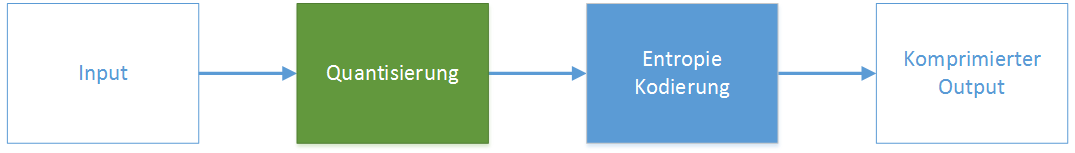
\includegraphics[width=0.8\textwidth,height=6cm,keepaspectratio]{./pictures/konzept/ist/aufbau.png}
	\caption{Aufbau der Ist-Kompression.}
	\label{konzept:ist:aufbau:diagramm}
\end{figure} 
Die Ist-Kompression führt zuerst ein Subsampling durch. Drei Viertel aller Punkte werden in diesem Schritt verworfen. Im nächsten Schritt werden die übrigen Punkte  auf 16-Bit Integer diskretisiert. Das reduziert die Anzahl Bytes und verbessert die Kompression im Schritt Entropie Kodierung. Die Implementationen der Entropie Kodierer scheinen Integer-Werte einfacher komprimieren zu können. In der Entropie Kodierung werden die Daten geordnet. Alle X-Kanäle der Feldlinien werden hintereinander abgelegt, gefolgt von allen Y-Kanälen etc. Diese Anordnung verbessert die Kompressionsrate der Entropie Kodierung. Je näher ähnliche Muster beieinander liegen, desto besser können sie Komprimiert werden. Für die eigentliche Entropie-Kodierung wird Gzip verwendet. Gzip basiert auf dem Deflate Algorithmus, welcher aus einer Kombination von LZ77 und Huffman Kodierung besteht \cite{wiki:gzip}.\\
Da die Punktmenge für Low-End Grafikkarten zu gross ist, führt der JHelioviewer ein weiteres Subsampling durch, welches im Abschnitt \ref{konzept:loesung0:subsampling} beschrieben ist.

\subsection{Lösungsansatz: Adaptives Subsampling} \label{konzept:loesung0}
\begin{figure}[!htbp]
	\center
	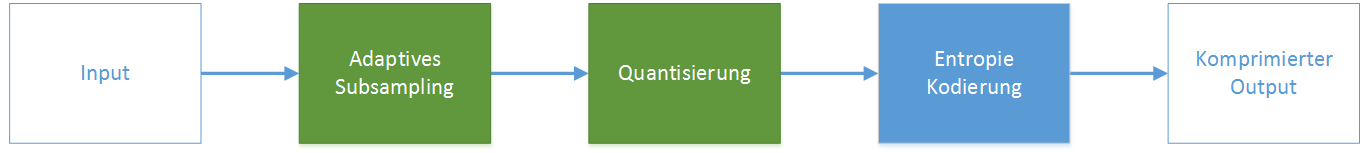
\includegraphics[width=0.8\textwidth,height=6cm,keepaspectratio]{./pictures/konzept/solution0/aufbau.png}
	\caption{Aufbau des Lösungsansatzes: Adaptives Subsampling.}
	\label{konzept:loesung0:aufbau:diagramm}
\end{figure} 
Dieser Lösungsansatz verwendet die selbe Pipeline wie die Ist-Kompression \ref{konzept:ist-komprimierung}. Der Unterschied ist, dass ein anderes Subsampling Verfahren gewählt wurde und eine andere Entropie-Kodierung. Die Abbildung \ref{konzept:loesung0:aufbau:diagramm} zeigt den neuen Ablauf. 

\subsubsection{Adaptives Subsampling}\label{konzept:loesung0:subsampling}
Ziel des adaptiven Subsamplings ist es, die Daten durch eine Folge von Strecken zu approximieren. An stellen, welche die Feldlinie gekrümmt ist, braucht es mehr Strecken. An Stellen, welche die Feldlinie Linear verlauft können so viele Punkte gespart werden. 
\begin{figure}[!htbp]
	\center
	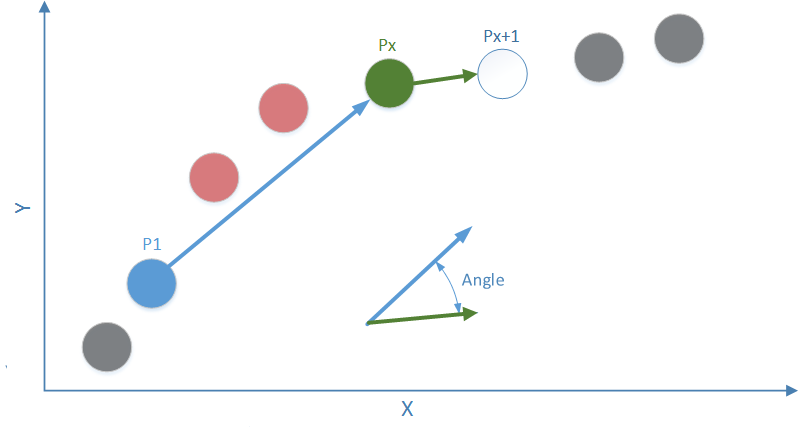
\includegraphics[width=0.8\textwidth,height=6cm,keepaspectratio]{./pictures/konzept/solution0/anglesubsampling.png}
	\caption{Darstellung des Adaptiven Subsapmlings im 2D Raum.}
	\label{konzept:loesung0:angle}
\end{figure}
Das Diagramm der Abbildung \ref{konzept:loesung0:angle} stellt das Subsampling im zweidimensionalen Raum dar. Zu sehen sind die Punkte der Feldlinie. Das Adaptive Subsampling wählt nun Punkte $P$ aus der Feldlinie aus, welche Start- und Endpunkte der Strecken darstellen.\\
$P_1$ wurde bereits ausgewählt. Es wird nun ein Punkt $P_x$ gesucht, der als Endpunkt einer Strecke von $P_1$ zu $P_x$ die Feldlinie approximiert. Dazu wird der Winkel der Strecke $P_1$ zu $P_x$ mit der Strecke $P_x$ zu $P_x+1$ verglichen. Wenn der Winkel kleiner ist, als ein Faktor $F$, wird der nächste Punkt $P_x+1$ überprüft. Wenn der Winkel grösser ist, wird $P_x$ ausgewählt und von $P_x$ aus weiter geprüft.

\subsubsection{Entropie Kodierung mittels RAR} \label{konzept:loesung0:kodierung}
Abspeicherung, Alle X Kanäle hintereinander, alle Y Kanäle etc. So kann die Entropide-Kodierung besser greifen.
Rar hat sich bewährt bei der purer Feldlinien kompression im Vergleich zu anderen Verfahren wie LZ77/gZip. Bringt etwa 4 mal bessere Kompression hin, hat aber mehr mühe mit Floating-Point nummern als mit Integers

\subsection{Lösung 1, Diskrete Kosinus Transformation}
Bild
DCT, da alles nahe an harmonischen Halbwellen

\subsubsection{Subsampling} \label{konzept:loesung1:subsampling}
Das Subsampling wurde aus der Ist-Kompression \ref{konzept:ist-komprimierung} übernommen und dient, die DCT zu beschleunigen. Da die DCT eine Komplexität von $O(n^2)$ aufweist, wird durch das Subsampling die Transformation wesentlich schneller.\\
Falls die Laufzeit der Dekompression weiter verbessert werden soll, kann die Fast-Cosine-Transformation umgesetzt werden. Diese hat eine Komplexität von $O(n log(n))$. Der Nachteil ist, dass nur Daten der Länge $2^n$ transformiert werden können, was zusätzliche Programmlogik braucht. Falls die Fast-Cosine-Transformation nicht ausreicht, können die Linien in Blöcken mit einer bestimmten Anzahl von Punkten unterteilt werden. Dadurch wird die Komplexität auf $O(n)$ gesenkt. Jedoch ist es wahrscheinlich, dass durch die Unterteilung die Kompressionsrate leidet. Vermutlich braucht es für die Approximation der Blöcke insgesamt mehr Kosinus-Funktionen, als für die Approximation der gesamten Feldlinie.\\

\subsubsection{Randbehandlung} \label{konzept:loesung1:randbehandlung}

\subsubsection{Principal Component Analysis}

\subsubsection{Cosinus-Transformation} \label{konzept:loesung1:kosinus}
Die Diskrete Kosinus Transformation stellt eine endliche Menge von $N$ Datenpunkten als $N$ Kosinusfunktionen zu verschiedenen Frequenzen dar. Die Werte DCT-Koeffizienten stellt dar, wie hoch der Anteil einer bestimmten Frequenz ist im Originalsignal. Im optimalen Fall kann ein Signal durch niederfrequente Funktionen approximiert werden. Die hochfrequenten Anteile stellen Details dar, welche nicht relevant sind.\\
Es gibt verschiedene Möglichkeiten die Punkte zu transformieren. . Es wurde sich am JPEG/JFIF Standard orientiert  , welcher, welche die DCT-II als Forwärts und die DCT-III als Rückwärtstransformation verwendet \cite{wallace1992jpeg}.
Der Unterschied liegt in der Randbehandlung

\begin{equation} \label{konzept:loesung1:kosinus:formula:fdct}
	X_k = \sum_{n=0}^{N-1}x_n cos[\frac{\pi}{N}(n+\frac{1}{2}k)] \quad k = 0, 1, \ldots, N-1
\end{equation}
$N$ ist anzahl Punkte. Transformiert in den Frequenzraum. $x_n$ ist ein Punkt des Signales und $X_k$ ist die Resultierende Kosinus Schwingung%? wirklich schwingung oder was anderes?

Inverse Transform
\begin{equation} \label{konzept:loesung1:kosinus:formula:idct}
X_k  = \frac{1}{2}x_0 + \sum_{n=1}^{N-1}x_n cos[\frac{\pi}{N}n(k+\frac{1}{2})] \quad k  = 0,1,\ldots,N-1
\end{equation}

\subsubsection{Quantisierung}


\subsubsection{Entropie Kodierung}\label{konzept:loesung1:kodierung}
Kodierung
	Idee: RUn length, fast alles nullen
	Adaptive

	Weitere Kodierung mittels Rar.
		Rar hat sich bewährt bei der purer Feldlinien kompression im Vergleich zu anderen Verfahren wie LZ77/gZip





